% Chapter Template

\chapter{Introduction} % Main chapter title

\noindent\textbf{\large Contents:}

\noindent\hrulefill
\noindent\startcontents[chapters]
\noindent\printcontents[chapters]{}{1}{}
\noindent\hrulefill

\label{Chapter1} % Change X to a consecutive number; for referencing this chapter elsewhere, use \ref{ChapterX}

Advances in astronomy come in many forms, from the exploration of new theories to new observational techniques.
But astronomy would not be possible without the main tool of the astronomer, the telescope.  Starting from when
Galileo Galilei first pointed his telescope to the night sky, astronomers have been demanding more from their
telescopes.  The only way to enhance a telescopes resolving power is to increase the primary aperture of the
telescope.  In the early 1900's telescopes were made up of a large single optics for the primary aperture. 
However, there is a limit to how large you can make a single optic.  


\begin{figure}[H]
\centering
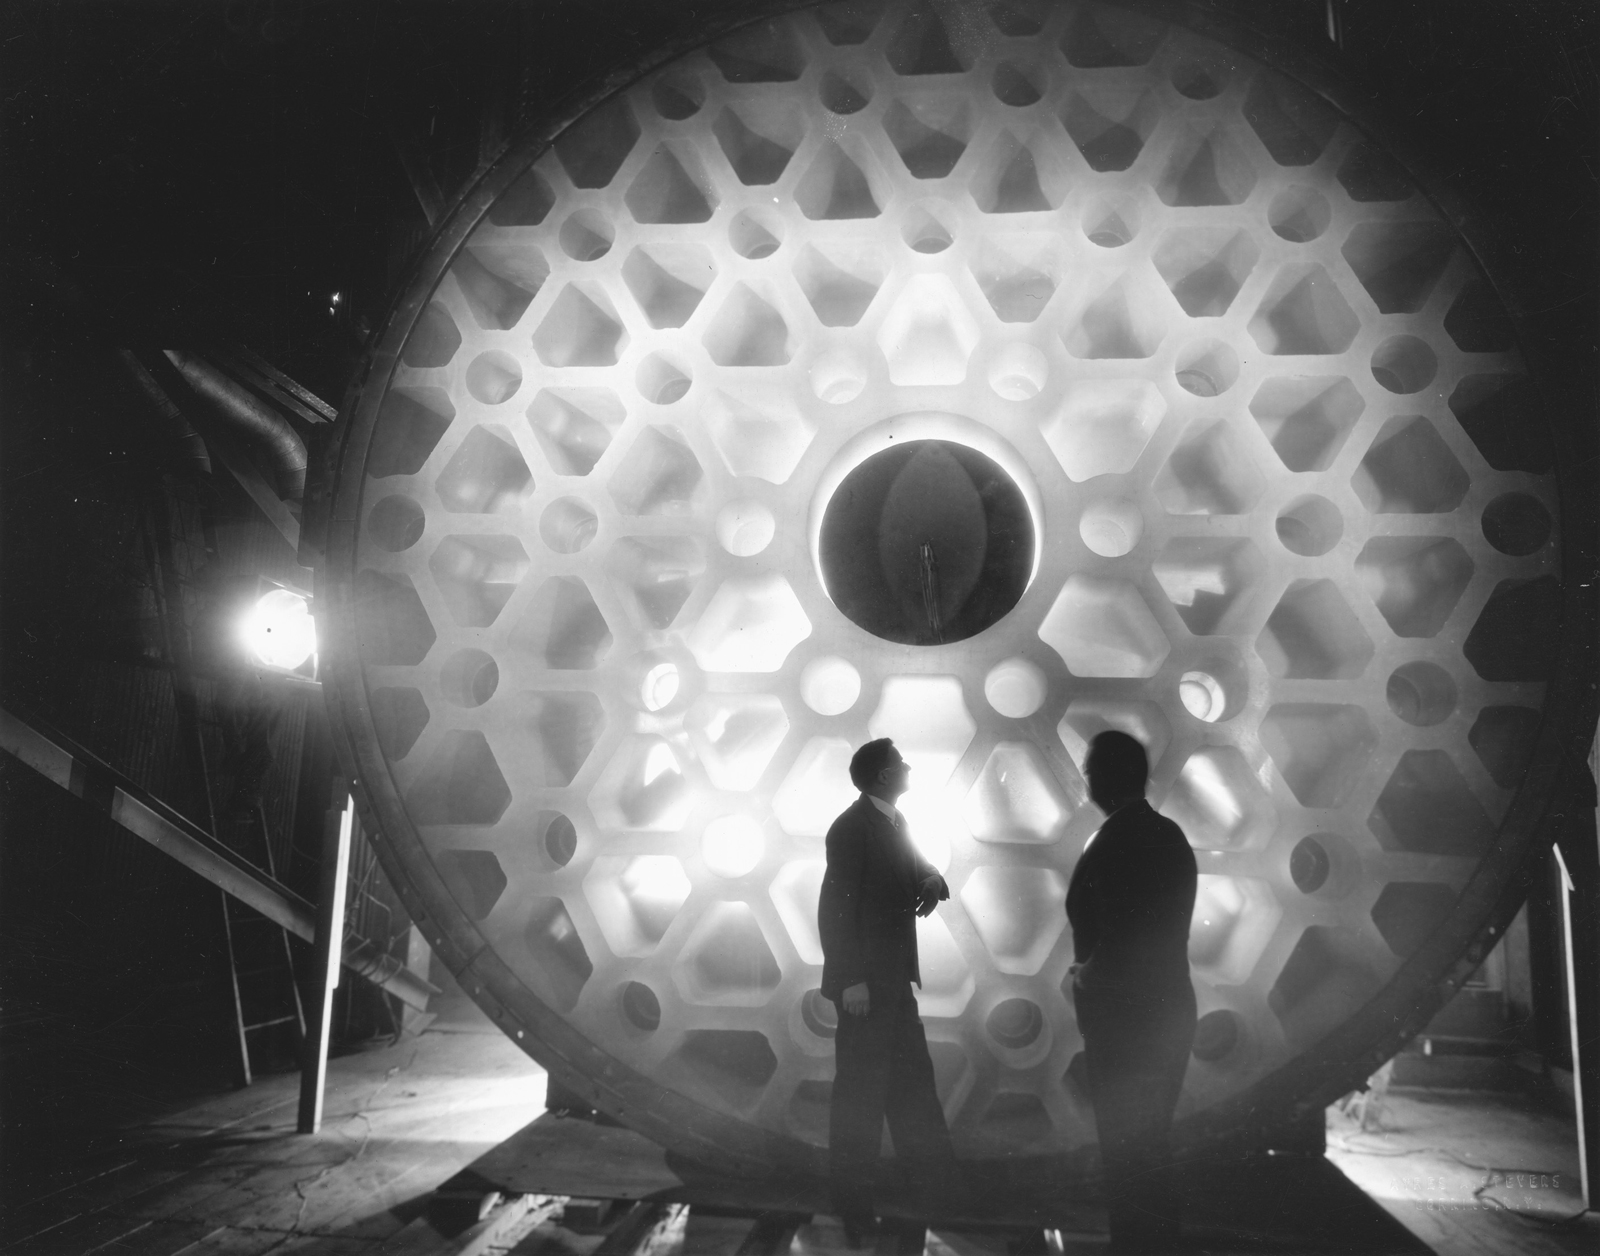
\includegraphics[width=12 cm]{../Figures/twomen}
\caption{Image of the Hale 200-inch (5.1m) primary mirror.  The honeycomb structure was to reduce the mass of the optic and make the surface more ridged}
\label{fig:hale}
\end{figure}

Eventually, these mirrors were becoming so
large that the mirrors would sag under their own weight.  These large optics quickly became heavier and needed
more mechanical supports.  In order to solve this problem, a honeycomb substructure was designed to keep the
mirrors lighter and more ridged.  Figure \ref{fig:hale} shows the primary mirror of the 200-inch Hale telescope
and backlight to show the structure.  While this helped keep large single optics rigid, there is still a limit
to how large one optic can be.  The University of Arizona's Large Optics Facility is capable of constructing
8.4 meter mirrors \cite{LOFTSystems.}.  One of the reasons for this limit is that this is roughly the maximum
width of bridge underpasses in Arizona.  In order to achieve larger primary apertures, a different approach is
needed.




\section{Segmented Mirrors / Active Optics}

In 1977, Dr. Jerry Nelson along with Dr. Terry Mast and a team of scientists at the Lawrence Berkeley National Laboratory, were tasked with designing a 10-meter telescope \cite{BeatingObservatory}.  The design they came up with was to use 36, 1.8 meter, hexagonal segments combined to make a 10-meter aperture (Figure \ref{fig:jerry_nelson}).  In order to make this work, all the segments needed to be aligned to sub-wavelength position.  This was accomplished by what is known as active optics.

\begin{figure}[H]
\centering
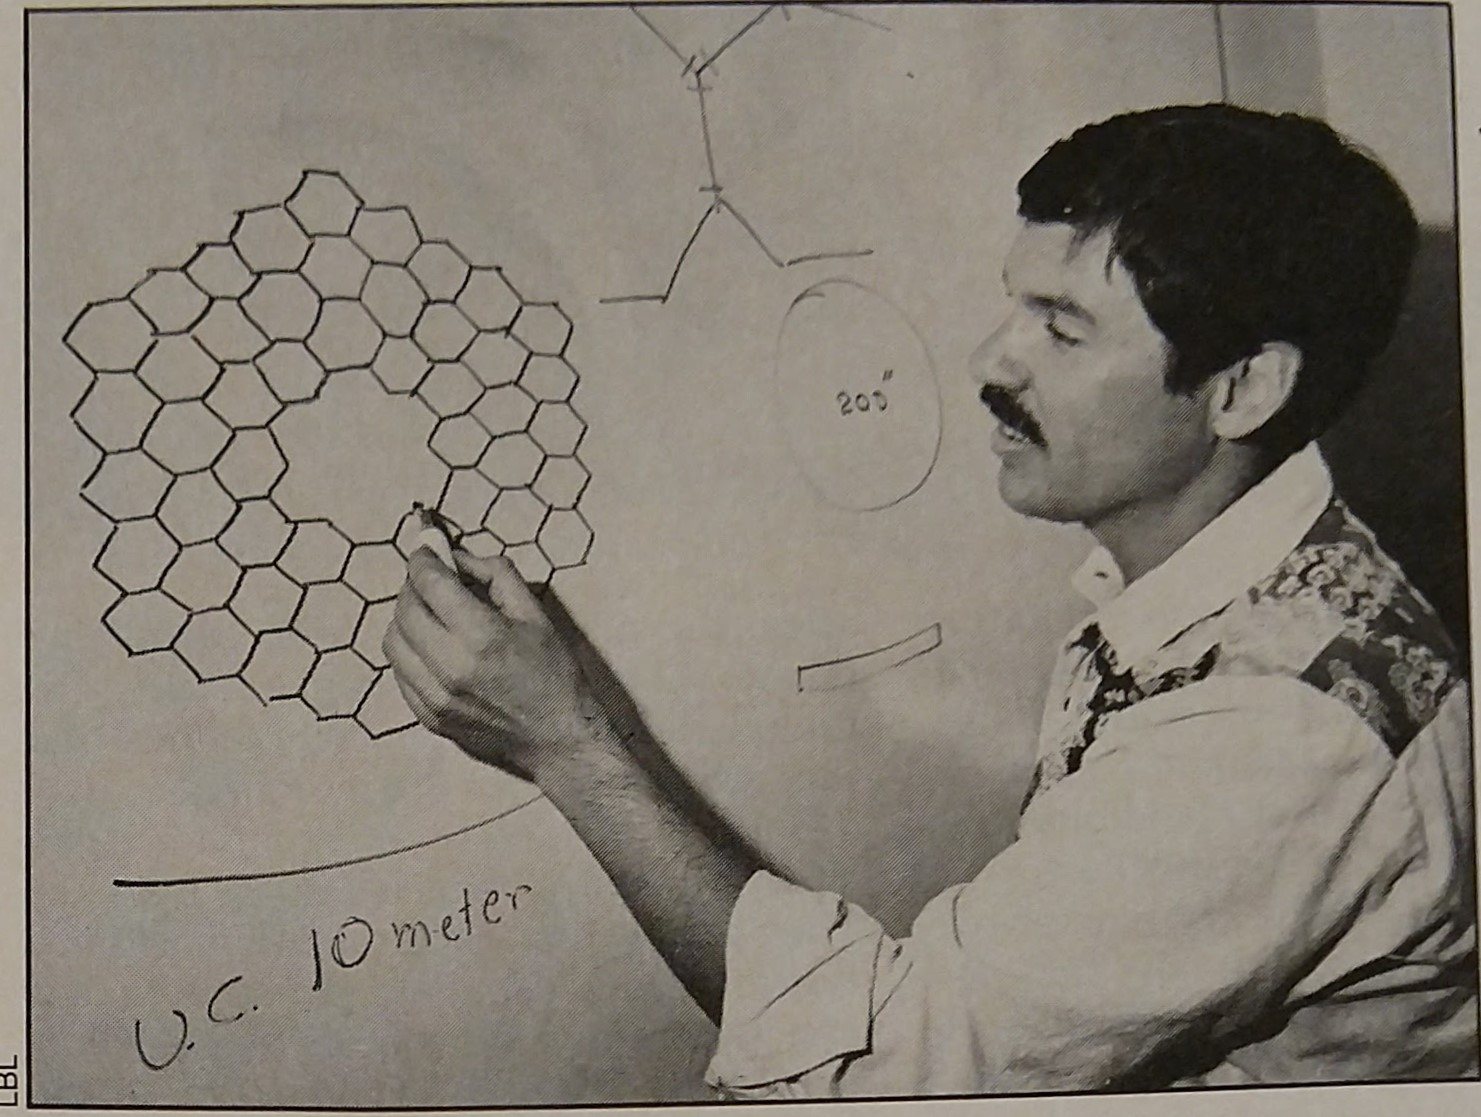
\includegraphics[width=12 cm]{../Figures/Jerry Nelson}
\caption{Jerry Nelson showing his segmented mirror design at Lawrence Berkeley Nation Laboratory.}
\label{fig:jerry_nelson}
\end{figure}

Active optics is the active control of each mirror segment so that all segments act as one large optic.  This is accomplished with nanometer level precision and differential capacitors to measure relative segment movement \cite{Nelson1990titleConstructionObservatory/title}.  This system is continuously running during observation and makes corrections from vibrations that the telescope may experience (i.e mechanical vibration, wind shake, etc).  The Keck position sensors are accurate to $\approx$ 30nm using differential capacitors.  A system view of the the Keck active optics can be seen in Figure \ref{fig:active_control}.


\begin{figure}[H]
\centering
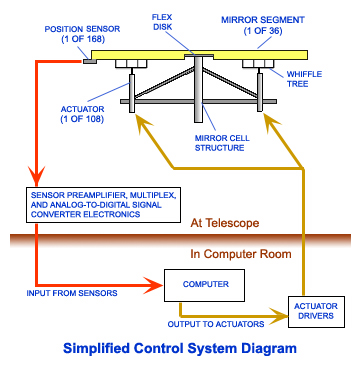
\includegraphics[width=12 cm]{../Figures/KCompDiag}
\caption{A system diagram of the Keck Telescope active control for a segment.}
\label{fig:active_control}
\end{figure}

Instead of hexagonal segments the Giant Magellan Telescope will be using seven, 8.4-meter, circular segments to make up it's 25 meter aperture.  





\section{FPWFS}



\section{Vector Apodizing Phase Plate}







%----------------------------------------------------------------------------------------
%	SECTION 1
%----------------------------------------------------------------------------------------
